%!TEX root = ../Thesis.tex
\chapter{Robot Hardware Daemon}
RHD (Robot Hardware Daemon) is the real-time hardware abstraction layer for the Mobotware platform, developed at DTU. RHD is a plugin-based platform that allows easy integration with sensors and actuators. RHD creates a synchronized database with read/write variables that can be shared between plugins and/or accessed by other software applications. RHD uses a real-time scheduler to ensure a fixed sample rate. \\
All setup of RHD is done based on a XML configuration file, containing all parameters and plugins specific to the robot. Plugins are intended to be general and works across robots, and all "magic" variables are placed in the configuration file.\\

\noindent
This project has been implemented as a configuration in RHD and plugins for hardware has been developed. To run the program type in:
\begin{lstlisting}[language=bash]
rhd trunk/plugins/tcuav/rhdconfig.xml
\end{lstlisting}
This runs the RHD program and loads the configuration for the Ground Control Station.


\section{Plugins}

\subsection{PhidgetsBridge2}
PhidgetBridge2 is build on the initial Phidgets Bridge plugin, only made more flexible by allowing the configuration file to contaion all of Phidgets Bridge configuration settings. The Phidget Bridge is a 4 channel amplifier, and is intended for measuring small voltages for example in loadcells. 

Configuring the bridge is done by first enabling the wanted channels. The default amplifier gain is 128V/V. The minimum sample time is 10 milliseconds. Calibration constant offset and gain is found by $F_{Exspected} = K*(Messured - Offset)$.

\begin{lstlisting}[language=XML]
<!-- Phidget Bridge -->
    <phidgetsbridge2
	    enable = "true"
	    lib="phidgetsbridge2.so.1"
	    debug = "1"
	    interval = "0"
	    updateTimeMs = "10"
	    gain = "128 128 128 0"
	    enableCh = "1 1 1 0"
	    offset = "-290 6050 -90 0"
	    k = "876 870 360 1"
      >
    </phidgetsbridge2>  
    
    <!-- Flight Control System - Tether Control of UAV -->
    <fcs 
	    enable= "true"
	    lib="fcs.so.1"
	    debug = "true"
      >
    </fcs>  
\end{lstlisting}

This plugin depends on Phidgets Linux Library. Special installation notes are found in the readme file.\\

\noindent
Files:
\dirtree{%
.1 plugins.
.2 phidgetsbridge2.
.3 99-phidgets.rules.
.3 Makefile.
.3 README.
.3 libphidget\_2.1.8.20140319.tar.gz.
.3 phidgetsbridge2.c.
.3 phidgetsbridge2.h.
.3 rhdconfig.xml.
}

\subsection{TCUAV}
TCUAV or Tether Control of UAV is the Ground Station.
\todo{Skriv}

\subsection{FCS}
FCS or Flight Control System is a part of the Tether Control of UAV project. This plugin establish contact to Ground Station via a Socket connection, and exchange information(references) from the ground stations measurements and control parameters, and then sends control parameters in to a PixHawk. It also reads 3 loadcell from a Phidget Bridge to determine the yaw and the force from the cable in x,y and z direction.\\
It is intended the PixHawk runs it's own position estimator in hard real time, and the control parameters from this plugin in soft real time, because of the variable delay in the feedback from the Ground Station.\\

\noindent
Setting up this plugin requires the PhidgetBridge2 to be configured first. 

\noindent
\begin{lstlisting}[language=XML]
<!-- Phidget Bridge -->
    <phidgetsbridge2
	    enable = "true"
	    lib="phidgetsbridge2.so.1"
	    debug = "1"
	    interval = "0"
	    updateTimeMs = "10"
	    gain = "128 128 128 0"
	    enableCh = "1 1 1 0"
	    offset = "-290 6050 -90 0"
	    k = "876 870 360 1"
      >
    </phidgetsbridge2>  
    
    <!-- Flight Control System - Tether Control of UAV -->
    <fcs 
	    enable= "true"
	    lib="fcs.so.1"
	    debug = "true"
      >
    </fcs>  
\end{lstlisting}

\noindent
This plugin depends on the phidgetsbridge2 plugin.\\

\noindent
Files:
\dirtree{%
.1 plugins.
.2 fcs.
.3 Makefile.
.3 fcs.c.
.3 fcs.h.
}

\subsection{RHDLink}
This plugin creates a socket connection to another RHD server(Server) and makes a copy of the variable database on the local machine(Client). The client with this plugin installed can access read and write variables on the other RHD server it is connected to, but the server can not read or write in the clients variable database. 
The Plugin is based on a copy of librhd.c, with a few alternations in the function and variable names to avoid name conflict. Only one RHD link per RHD server can run without conflicts. \\

\noindent
The configuration of the plugin is done in the XML file ''rhdconfig.xml'' and adding following to the plugin configuration. Substitutting host and port to the corresponding RHD server will access another server weather it's on the local machine or on the network.
The access rights can be set as read(r) or write(w), if write both read and write are possible.
\begin{lstlisting}[language=XML]
<!-- *** RHD Link - creates a link to another RHD server *** -->
<rhdlink enable="true"
	  lib="rhdlink.so.1"
      host="192.168.7.2"
      port="24902"
      access="w"
      debug="true">
</rhdlink>
\end{lstlisting}

\noindent
This plugin requires the RHD component of Mobotware version 3.583.\\

\noindent
Files:
\dirtree{%
.1 plugins.
.2 rhdlink.
.3 Makefile.
.3 librhdlink.c.
.3 librhdlink.h.
.3 rhdconfig.xml.
.3 rhdlink.c.
.3 rhdlink.h.
}


\subsection{Joycontrol}
This plugin provides remote override control possibilities using a standard HID Joystick. The plugin is developed by Anders Billso Beck and automatic detect the vehicle steering configuration for wheel based robots. For this project the plugin was modified to be able to detect UAV steering parameters. The plugin detect the steering configuration on which unique control variables it can find in the variable database. UAV steering has unique control variables like yaw, pitch, roll and height.


\begin{figure}[hbtp]
\centering
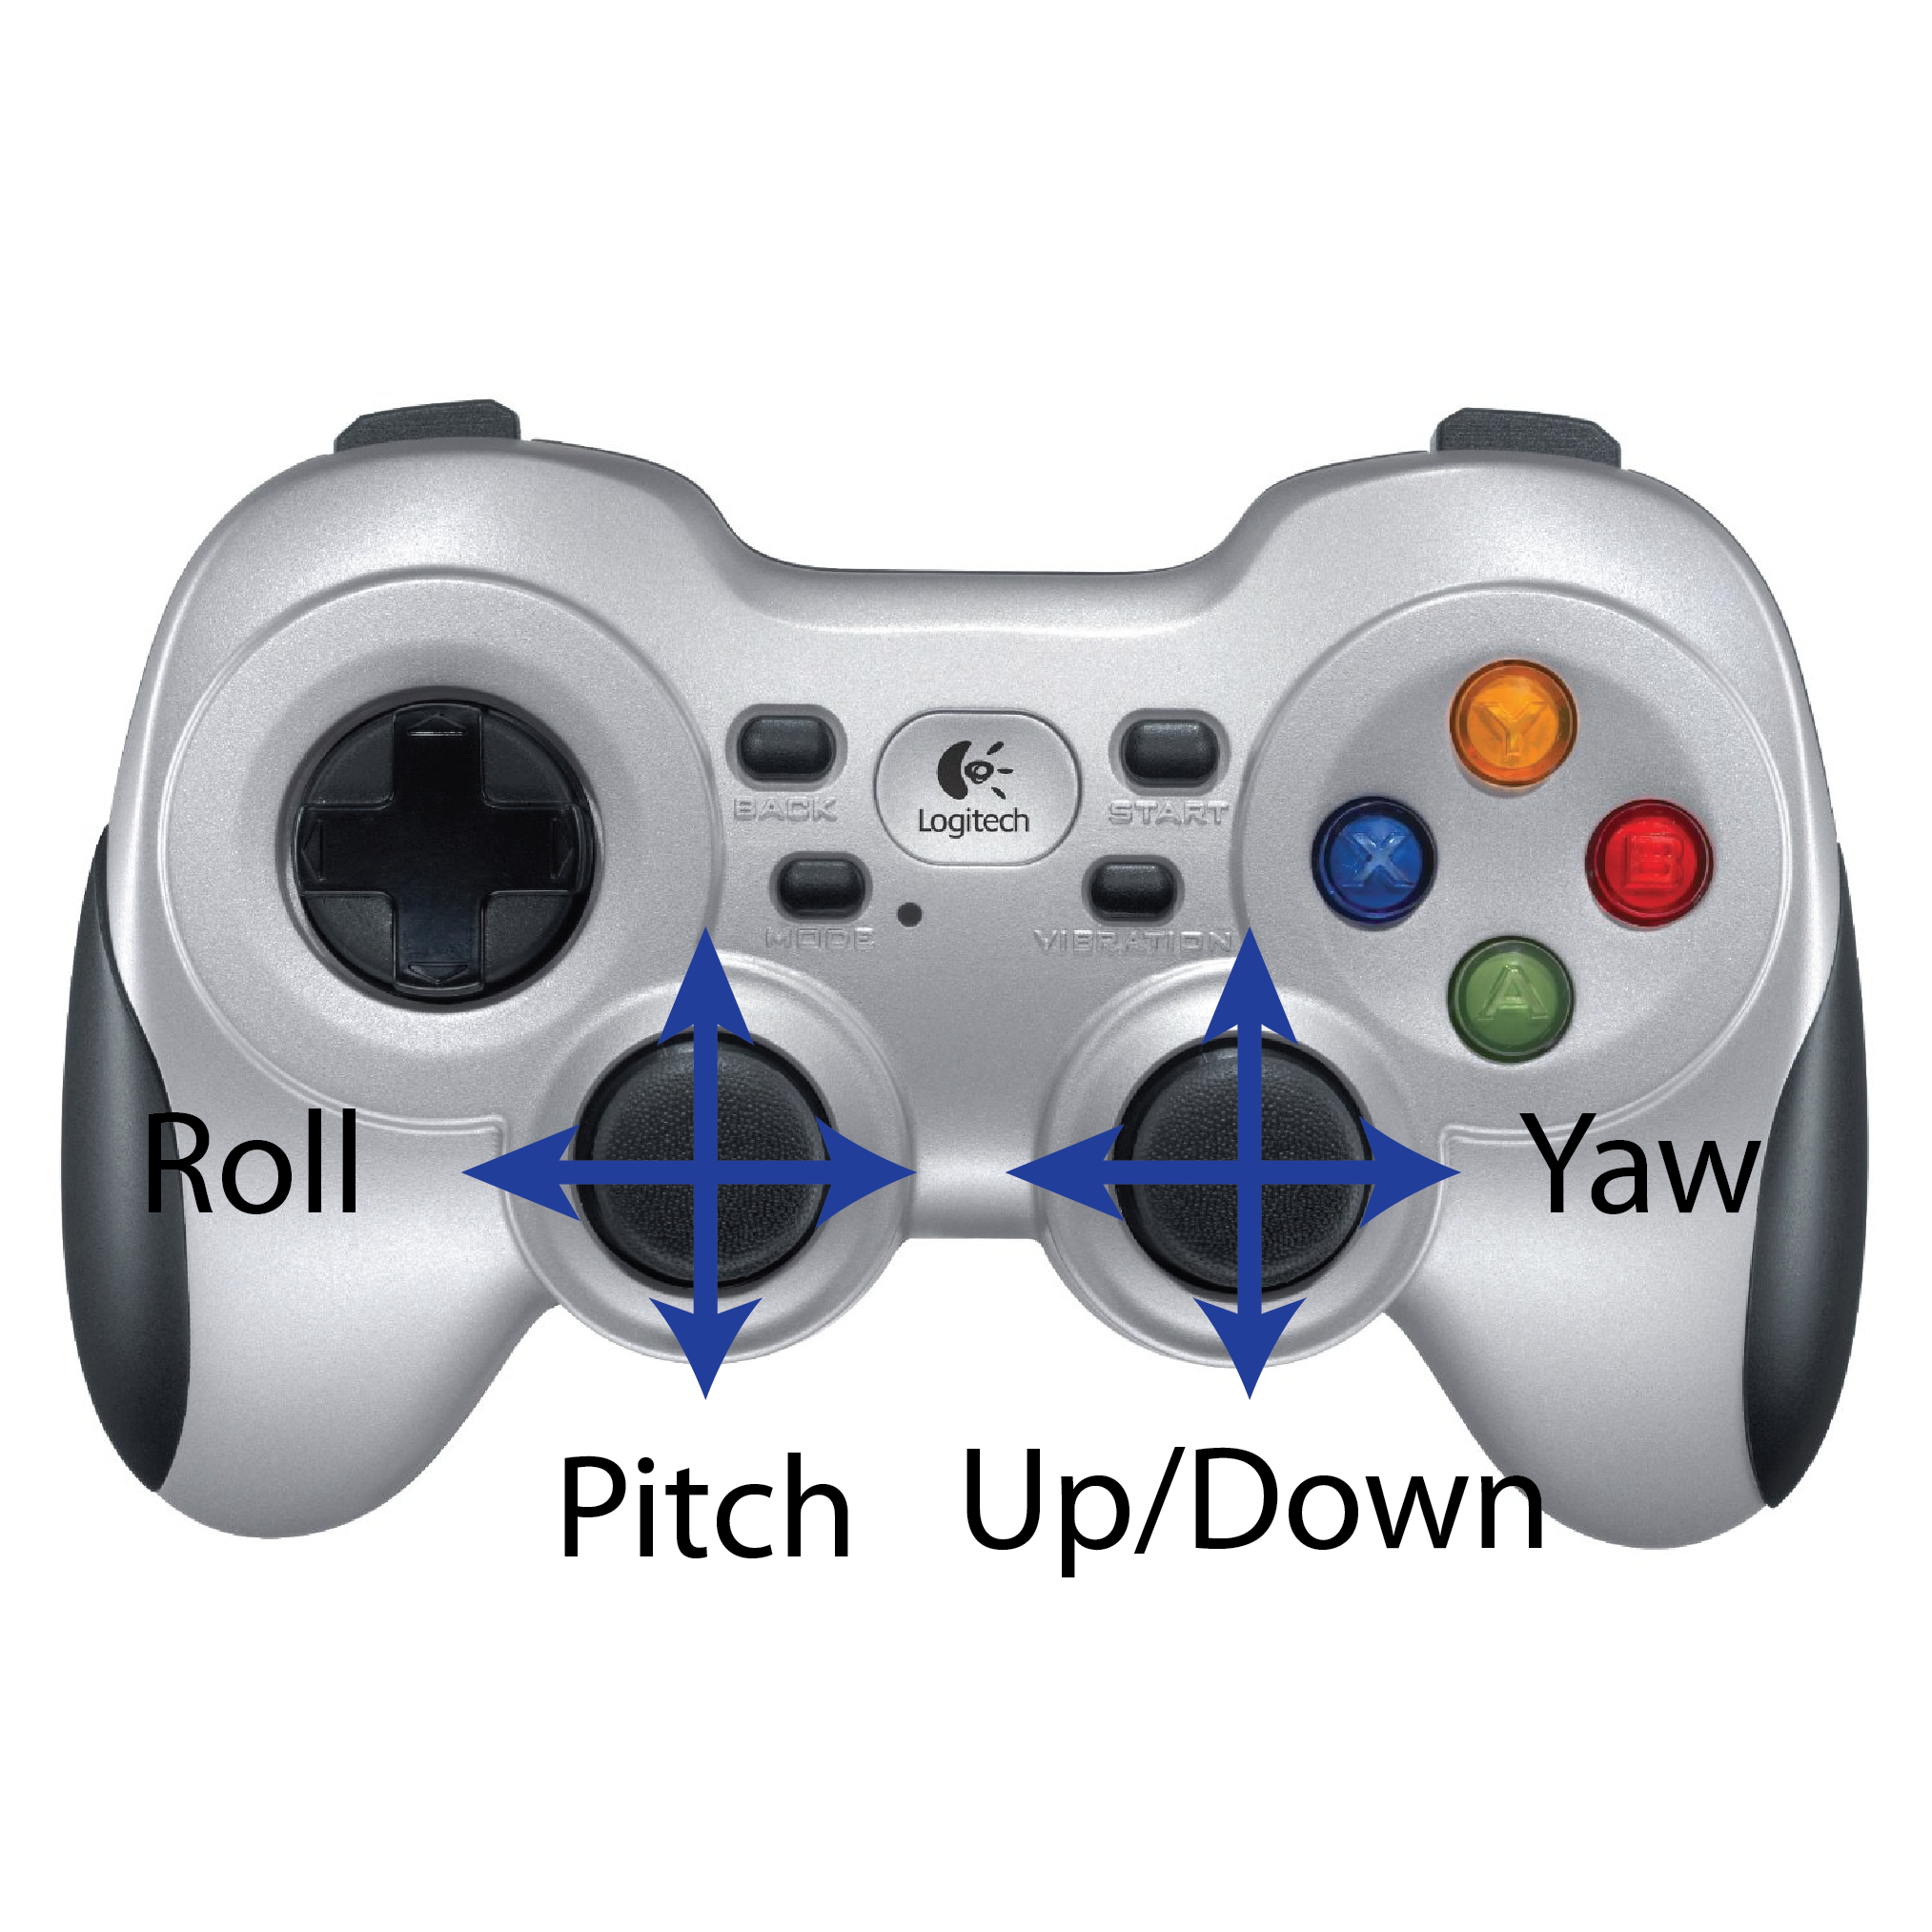
\includegraphics[scale=0.5]{graphics/joycontrol/joycontrol.png}
\caption{Implementation of joystick control for UAV control.}
\end{figure}

\noindent
Files:
\dirtree{%
.1 plugins.
.2 joycontrol.
.3 Makefile.
.3 joycontrol.c.
.3 joycontrol.h.
}  

